\documentclass{beamer}
\usetheme{Rochester}
\usecolortheme{default}
%\setbeamercolor{structure}{fg=black}
\beamertemplatenavigationsymbolsempty

\usepackage[ngerman]{babel}
\usepackage{graphics}
\usepackage{mathtools}
\usepackage{amsmath}

\title{Word2Vec und das Skip-Gram-Modell von Grund auf skripten: Eigene Word Embeddings erstellen}
\author{Aleksandr Schamberger}
\institute{Humboldt-Universität zu Berlin\\Institut für Slawistik und Hungarologie\\Sprachenübergreifend: Computerlinguistik II – Digitale Sprachmodelle und ihre Anwendung\\Sommersemester 2024}
\date{\today}

\AtBeginSection[]{%
	\begin{frame}
		\frametitle{Gliederung}
		\tableofcontents[currentsection]
	\end{frame}
}

\begin{document}

\frame{\titlepage}

\begin{frame}[t]{Gliederung}
\tableofcontents
\end{frame}


\section{Wörter (sinnvoll) als Zahlen darstellen}

\begin{frame}[c]{Wörter (sinnvoll) als Zahlen darstellen}
\begin{itemize}
	\item Bank
	\item Stuhl
	\item Sitzgelegenheit
	\item dick
	\item dünn
	\item schlank	
\end{itemize}
\end{frame}

\begin{frame}[c]{ASCII-Tabelle}
	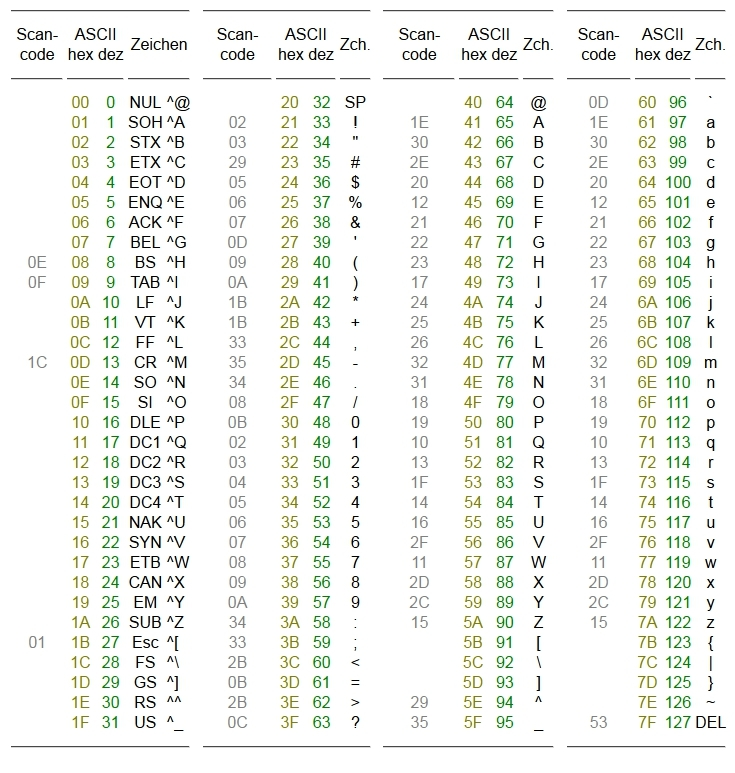
\includegraphics[scale=0.3]{"../pics/ASCII_Tabelle.jpeg"}
\end{frame}

\begin{frame}[c]{Wörter als deren ASCII-Zeichenkodierung}
	\begin{itemize}
		\item Bank
		\begin{itemize}
			\item 66 97 110 107 10 
		\end{itemize}
		\item Stuhl
		\begin{itemize}
			\item 83 116 117 104 108 
		\end{itemize}
		\item Sitzgelegenheit
		\begin{itemize}
			\item 83 105 116 122 103 101 108 101 103 101 110 104 101 105 116 
		\end{itemize}
		\item dick
		\begin{itemize}
			\item 100 105 99 107 
		\end{itemize}
		\item dünn
		\begin{itemize}
			\item 100 195 188 110 110 
		\end{itemize}
		\item schlank
		\begin{itemize}
			\item 115 99 104 108 97 110 107 
		\end{itemize}
	\end{itemize}
\end{frame}

\begin{frame}[c]{Semantische Relationen (und Eigenschaften)}
	\begin{itemize}
		\item \textbf{Hyponymie/Hyperonymie}: (Bank,Stuhl) $\rightarrow$ Sitzgelegenheit
		\item \textbf{Ko-Hyponymie}: Bank - Stuhl
		\item \textbf{Antonymie}: dünn - dick
		\item \textbf{Synonymie}: dünn - schlank
		\item \textbf{Ambiguität}: Bank - Bank
	\end{itemize}

\vspace{0.5cm}

\onslide<2->{Und viele weitere, sprachliche Eigenschaften $\ldots$}
\end{frame}

\begin{frame}[c]{Zwischenlösung: One-Hot-Vektoren}
\begin{itemize}
	\item Bank
	\begin{itemize}
		\item 1 0 0 0 0 0
	\end{itemize}
	\item Stuhl
	\begin{itemize}
		\item 0 1 0 0 0 0
	\end{itemize}
	\item Sitzgelegenheit
	\begin{itemize}
		\item 0 0 1 0 0 0
	\end{itemize}
	\item dick
	\begin{itemize}
		\item 0 0 0 1 0 0
	\end{itemize}
	\item dünn
	\begin{itemize}
		\item 0 0 0 0 1 0 
	\end{itemize}
	\item schlank
	\begin{itemize}
		\item 0 0 0 0 0 1 
	\end{itemize}
\end{itemize}
\end{frame}

\begin{frame}[c]{Problem: Der Umfang des deutschen Wortschatzes}
	
Umfang deutscher Wörter (Grundformen)

\vspace{0.5cm}

	\begin{itemize}
		\item<2-> Aktiver Wortschatz: 12.000 - 16.000
		\item<3-> Passiver Wortschatz: 50.000
		\item<4-> Im Allgemeinen angenommen: 300.000 - 500.000
		\item<5-> Dudenkorpus: > 18 Millionen
	\end{itemize}

\vspace{0.5cm}

\onslide<6->{10.000 Wörter: Bank $\rightarrow$ $1_1 0_2 0_3 0_4 0_5 0_6 0_7 0_8 0_9 \ldots 0_{10.000}$}
\end{frame}



\section{Worteinbettungen (Word Embeddings)}

\begin{frame}[c]{Von weiten Vektoren zu dichten Vektoren}
	10.000 Wörter: Bank $\rightarrow$ $1_1 0_2 0_3 0_4 0_5 0_6 0_7 0_8 0_9 \ldots 0_{10.000}$
	
	\onslide<2->{
	
	\vspace{0.5cm}
	
	$\leftrightarrow$
	
	\vspace{0.5cm}
	
	10.000 Wörter: Bank $\rightarrow$ $-1,23_1 3,4_2 0,09_3 0_4 1,1_5 0,98_6 -2,34_7 0,11_8 -1,3_9 \ldots 0_{300}$}
\end{frame}

\begin{frame}[c]{Skip-Gram-Modell: Gesamtmodell mit Beispielrechnung}
	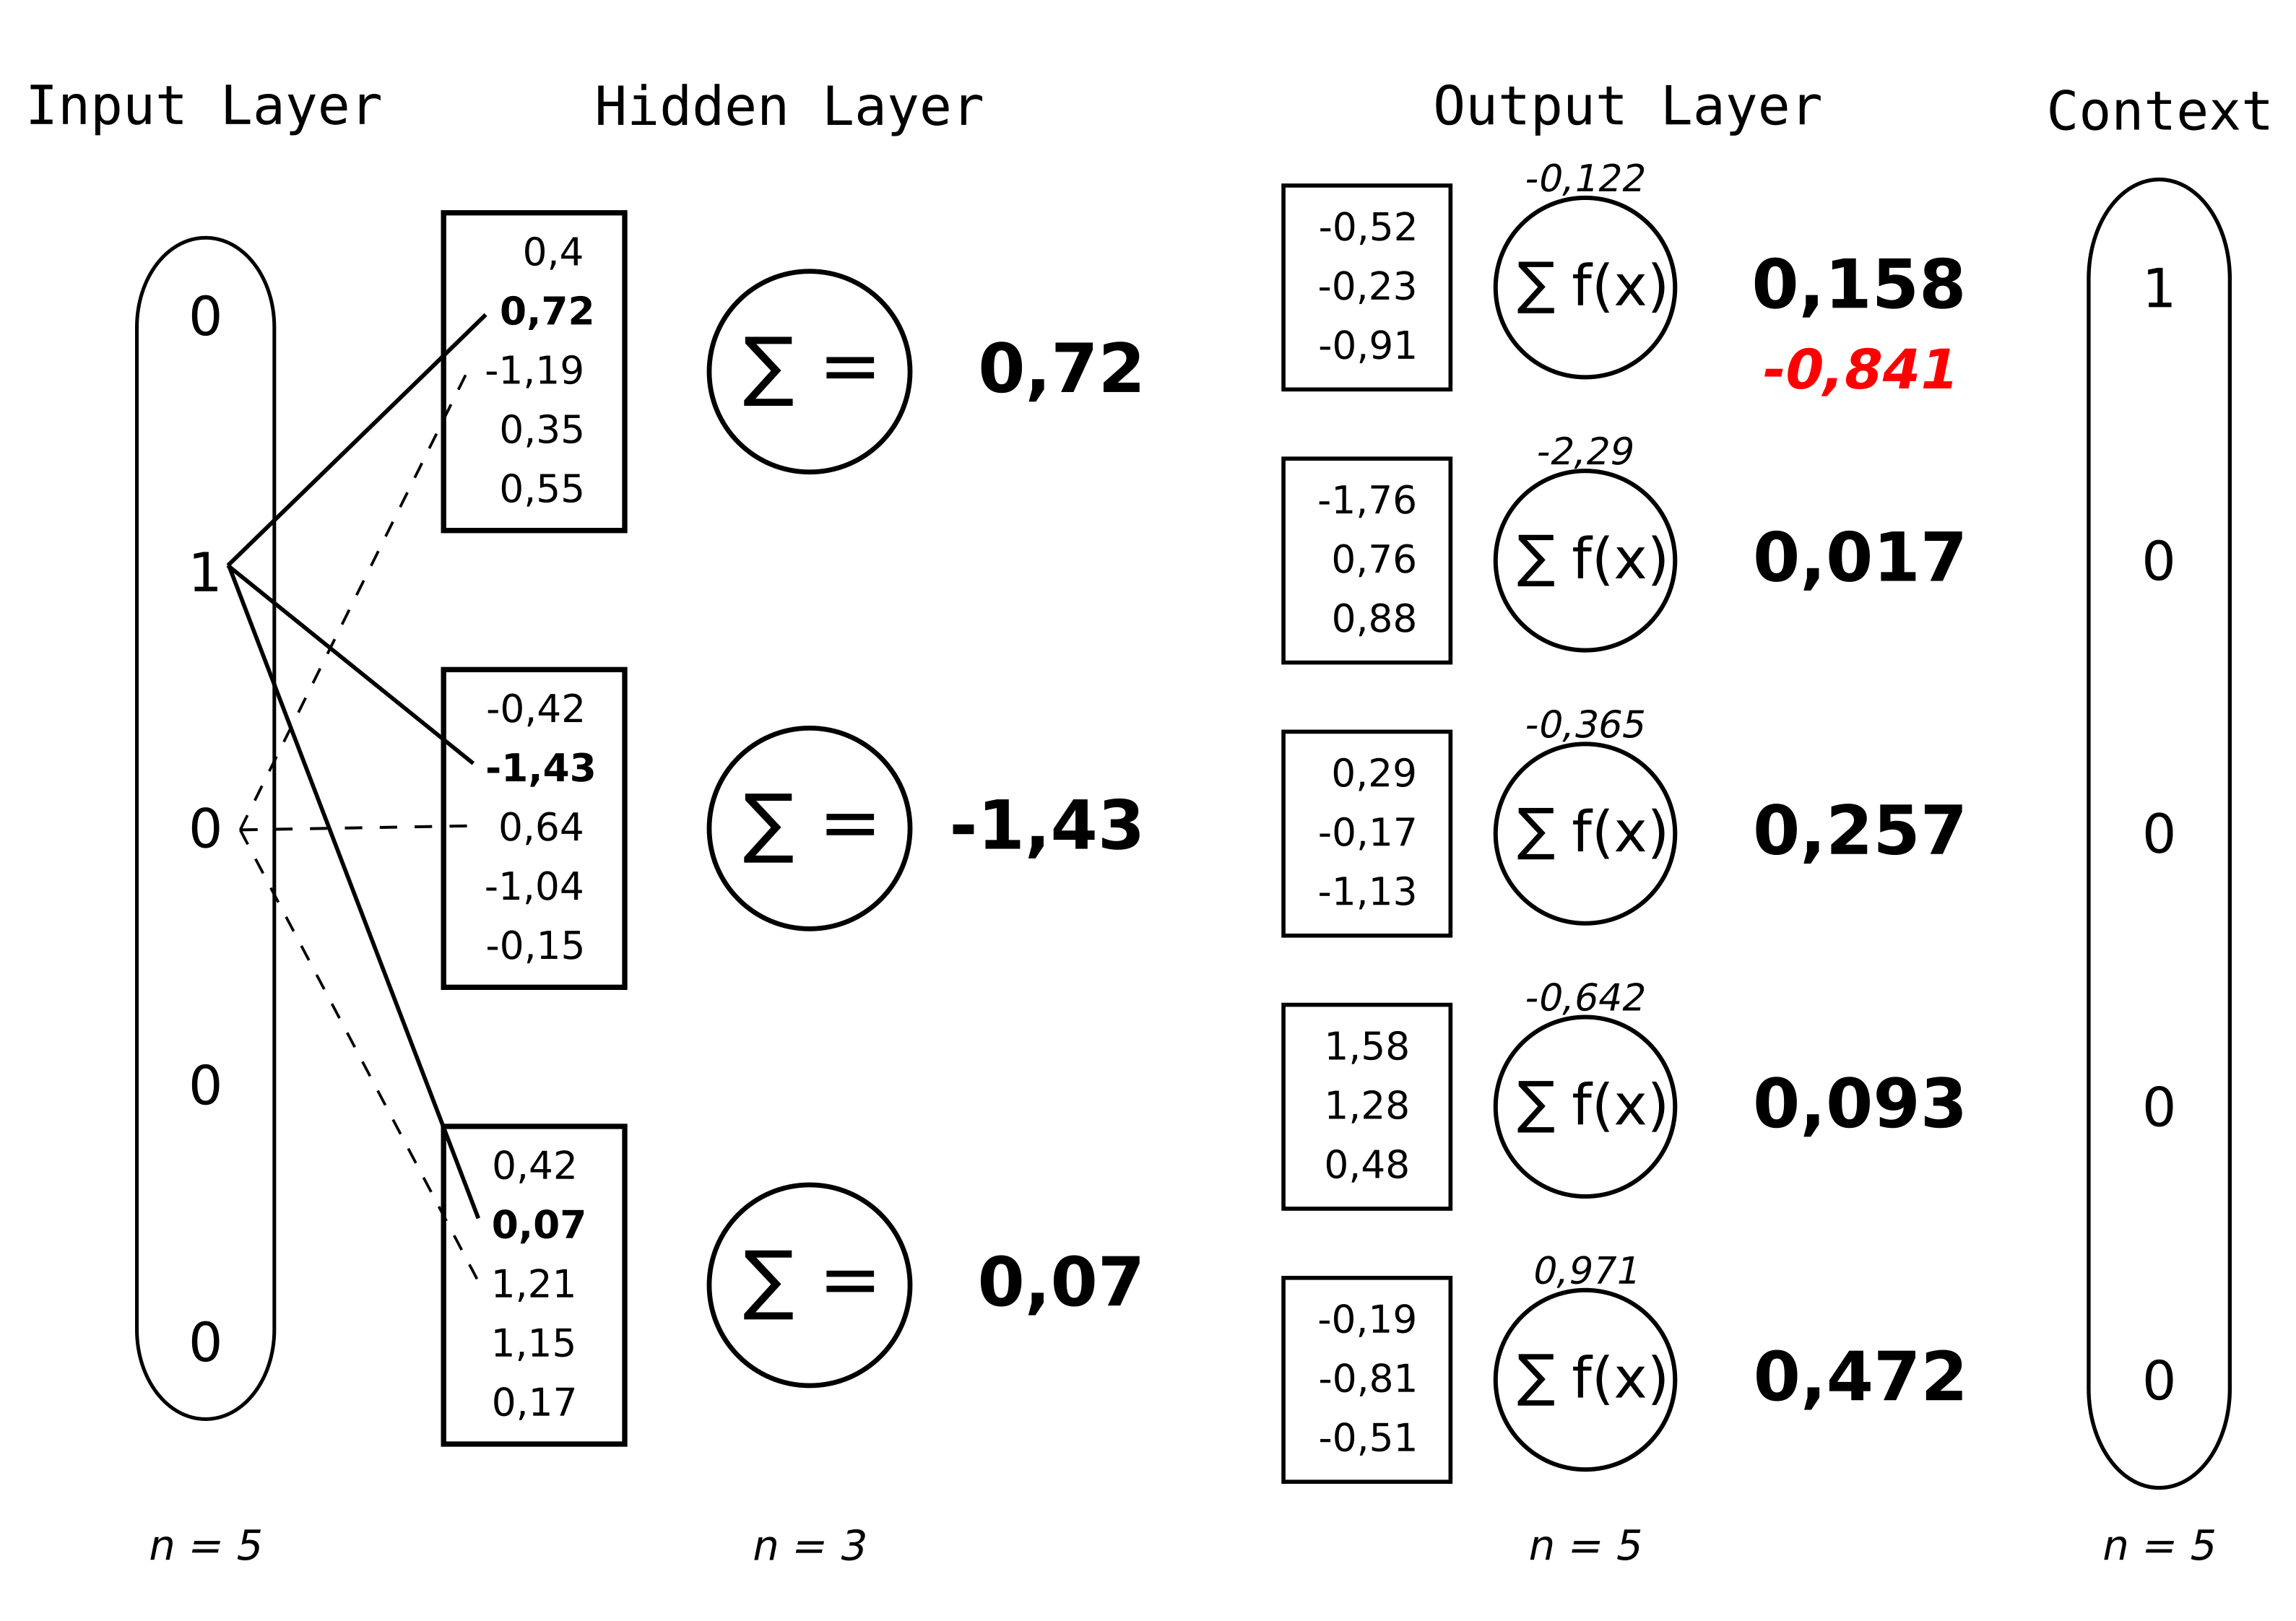
\includegraphics[scale=0.13]{"../pics/word2vec_skipgram_graphics.png"}
\end{frame}

\begin{frame}[c]{Skip-Gram-Modell: Kontext (Syntagma)}
	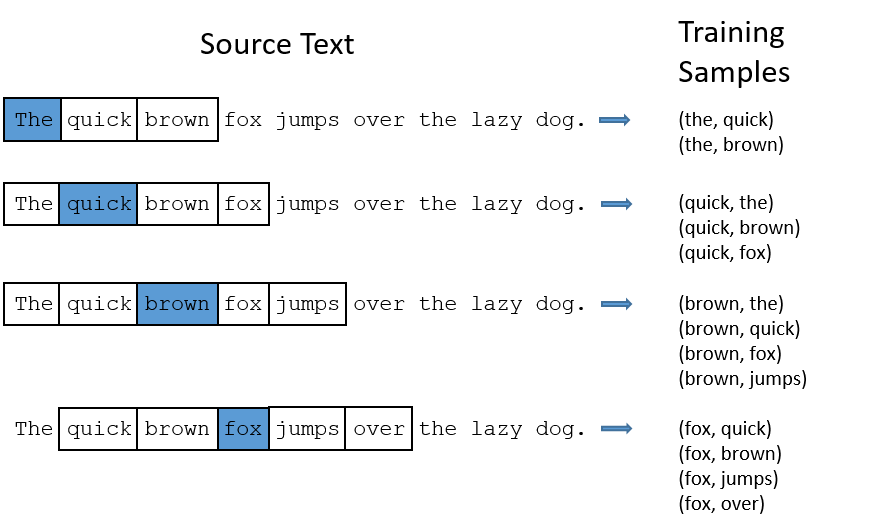
\includegraphics[scale=0.8]{"../pics/training_data_context.png"}
\end{frame}

\begin{frame}[t]{Quellen}
	\begin{itemize}
		\item Tae, Jake (13.07.2020): Word2vec from Scratch <https://jaketae.github.io/study/word2vec/> (abgerufen am 02.07.2024)
		\item McCormick, Chris (19.04.2016): Word2Vec Tutorial - The Skip-Gram Model <http://mccormickml.com/2016/04/19/word2vec-tutorial-the-skip-gram-model/> (abgerufen am 02.07.2024)
		\item Tae, Jake (05.02.2020): Building Neural Network From Scratch <https://jaketae.github.io/study/neural-net/> (abgerufen am 02.07.2024)
		\item Tae, Jake (21.12.2019): Demystifying Entropy (And More) <https://jaketae.github.io/study/information-entropy/> (abgerufen am 02.07.2024)
	\end{itemize}
\end{frame}


\begin{frame}[c]{Skip-Gram-Modell: Beispiele}
	\begin{center}\Large{\textbf{Beispiel(e) im Editor!}}\end{center}
\end{frame}

\end{document}

